\documentclass[runningheads]{llncs}
%
\usepackage{silence}
\usepackage{graphicx}
\usepackage{mathtools}
\DeclarePairedDelimiter{\ceil}{\lceil}{\rceil}
\DeclarePairedDelimiter{\floor}{\lfloor}{\rfloor}
\begin{document}
%
\title{Agrupamiento jerárquico balanceado para el problema de enrutamiento de flotas}
%
%\titlerunning{Abbreviated paper title}
% If the paper title is too long for the running head, you can set
% an abbreviated paper title here
%
\author{Juan José Sapuyes Pino, \and
    Juan Manuel Pajoy López \and
    Juan Pablo Ortega Medina \and
    Sebastián Rendón Giraldo.}
%
\authorrunning{}
% First names are abbreviated in the running head.
% If there are more than two authors, 'et al.' is used.
%
\institute{Universidad Nacional de Colombia, Medellín, Colombia.
    \email{\{jsapuyesp,jpajoyl,jportegame,serendongi\}@unal.edu.co}}
%
\maketitle% typeset the header of the contribution
%
\begin{abstract}
    Este artículo propone un método de agrupamiento jerárquico geográfico para tratar de
    solucionar una parte del problema del enrutamiento de flotas, en este caso para
    laboratorios con tomas de muestras a domicilio. El algoritmo es un algoritmo
    jerárquico aglomerativo, que utiliza una filosofía bottom-up para el agrupamiento
    y de divide y vencerás para hallar los pares de grupos más cercanos.
    \keywords{Clústering  \and Agrupamiento \and Jerárquico.}
\end{abstract}

\section{Introducción}
Existen laboratorios que prestan el servicio de toma de muestras en casa,
un servicio bastante útil para personas que por alguna dificultad no pueden desplazarse
hasta el lugar donde se toman las muestras, estas muestras se toman y son transportadas
al laboratorio a bajas temperaturas, para poder preservarlas. Sin embargo, los laboratorios
que prestan estos servicios se encuentran con un gran problema, ¿cuál es la ruta óptima para
la persona que toma la muestra? Esto es un problema bastante recurrente para los laboratorios
y es de vital importancia resolverlo, pues las muestras se encuentran en neveras portátiles,
las cuales preservan las bajas temperaturas, pero no durante mucho tiempo.  Estos recorridos se
realizan en horas de la mañana, tomando como punto de partida el hogar del domiciliario $P_{0}$,
este debe visitar los diferentes lugares designados para la recolección de muestras $P_{r}$ y
finalizar el recorrido en el laboratorio $P_{e}$.
\\
Para determinar las rutas optimas para los domiciliarios, se realiza un proceso de agrupamiento
o clústering geográfico de los diferentes puntos de recolección $P_{r}$ por zonas \cite{bard11},
para esto se tiene en cuenta la cantidad de domiciliarios disponibles $K$, los cuales se encargarán
de tomar las muestras.
\\
Este procedimiento no sólo beneficiará a los laboratorios que presten estos servicios representando
menores costos logísticos y probablemente un mayor número de servicios diarios, sino también a los
domiciliarios encargados de tomar las muestras, pues tendrán rutas más consistentes diariamente y
recorrerán menores distancias.


\section{Planteamiento del problema}
Dado un conjunto de puntos de recolección de muestras $P_{R}$ con coordenadas
$(x, y)$ y una cantidad de enfermeros domiciliarios $K$ para un día de la semana,
necesitamos encontrar $K$ clusters de tamaño mínimo $\floor{\frac{R}{K}}$ y tamaño
máximo $\ceil{\frac{R}{K}}$.

El problema es un subproblema del enrutamiento de flotas, en el cuál debemos encontrar
los grupos geográficos que minimicen las distancias entre clientes, y asignar cada uno
de estos grupos a un enfermero. El problema de hallar la ruta óptima dentro de cada
grupo no se aborda en esta propuesta.
\subsection{Técnicas propuestas por otros autores}
Se han propuesto métodos de clústering geográfico para redes de recolección y entrega
de paquetes, que buscan minimizar el número de vehículos de la flota que
la empresa debe usar, utilizando algoritmos jerárquicos aglomerativos con una función
de distancia que logren minimizar los tiempos (costo) entre clientes de un clúster
\cite{bard11}.
\\
Nazari, et al. \cite{nazari19}, proponen un algoritmo \textit{bottom-up} de clústering
jerárquico con puntos superpuestos con complejidad $O(n^{2})$, agrupando parejas en cada nivel,
encontrando intersecciones entre clústers y creando un nuevo clúster como la unión de estos dos.
\section{Método}
Para la creación de los grupos, se va a utilizar un algoritmo aglomerativo, que implica que se
van a calcular los puntos más cercanos de todo el conjunto de puntos, que se irán juntando poco
a poco hasta formar grupos más grandes con la cantidad deseada. Esta distancia se va a calcular
teniendo en cuenta el algoritmo de divide y vencerás para la selección de estos puntos, armando
parejas de puntos lo más juntos posibles. Una vez se unan los puntos, se generará un punto medio,
que hará parte de la nueva lista de puntos, para así repetir el proceso.
\\
Al finalizar la seleción de los clusters, se hará la asignacion de los grupos a cada
uno de los domiciliarios, que se hace de manera iterativa sobre los domiciliarios disponibles.
Se comienza encontrando el clúster más cercano para todos los domiciliarios disponibles y en
caso de desempate, se seleccionará el domiciliario más lejano (para que la varianza de las
distancias domiciliario-clúster sea lo más baja posible).
\subsection{Algoritmo}
El pseudocódigo del algoritmo propueso es el siguiente:
\begin{verbatim}
clusters_completos = []
clusters = puntos_entrega
clusters_actuales = tamaño de clusters
mientras clusters_actuales < numero_domiciliarios):
    # Función para calcular los puntos más cercanos por medio de divide y vencerás
    pares_cercanos = pares_cercanos(puntos_entrega)
    clusters = pares_cercanos['puntos_sobrantes'] 
    punto_medio: pares_cercanos['pares']
    si tamaño del cluster con centroide en punto_medio >= numero_domiciliarios:
        agregar a clusters_completos el punto_medio
    sino:
        agregar a clusters el punto_medio
    restar 1 a clusters_actuales
\end{verbatim}
La complejidad de este algoritmo es de $O(N^2log^2(N))$, que es peor que el de otros métodos
de agrupación, sin embargo, es más preciso que otros métodos como K-means \cite{nazari19} y
creemos que esto compensa su peor eficiencia.
\section{Resultados}
El algoritmo es viable para un número de puntos de entrega no mayor a 100, lo
cual es viable para empresas con alrededor de 10 domiciliarios.
\\
\textbf{Nota}: las pruebas fueron realizadas en un MacBook Air M1 a 3,2 GHz.
\begin{figure}
    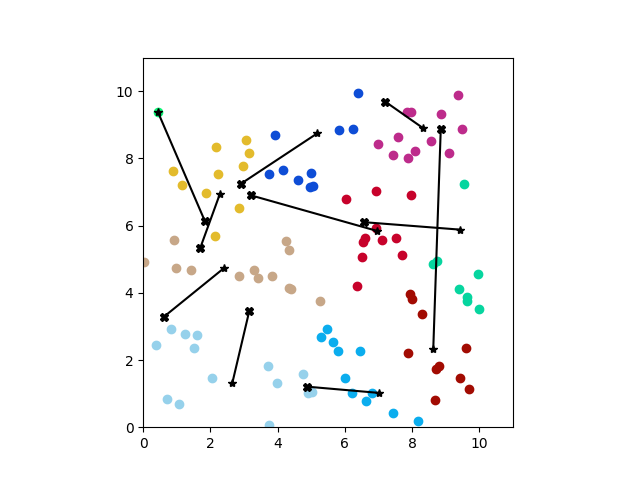
\includegraphics[width=\textwidth]{result_1.png}
    \caption{Resultados del algoritmo para 100 puntos de entrega y 10 domiciliarios.
        Tiempo de ejecución: 29,25 ms.}
\end{figure}
\begin{figure}
    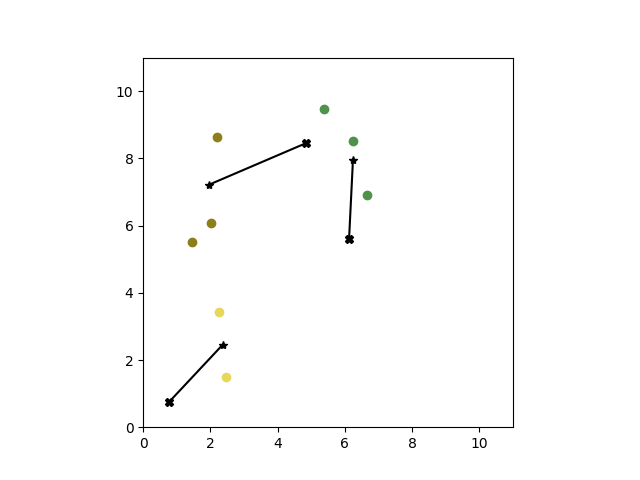
\includegraphics[width=\textwidth]{result_2.png}
    \caption{Resultados del algoritmo para 8 puntos de entrega y 3 domiciliarios.
        Tiempo de ejecución: 109,20 $\mu$s}
\end{figure}
\newpage
\section{Conclusiones}
El agrupamiento, en su mayoría genera resultados satisfactorios, sin embargo, es necesario
una mayor investigación para crear una versión modificada capaz de crear clusters más
balanceados.
\\
El algoritmo propuesto presenta una manera más precisa de agrupamiento que otros
algoritmos mencionados, y aunque su complejidad en tiempo sea mayor, puede ser útil
en casos donde se busque un agrupamiento más preciso.
\\
En este experimento se realizaron varios intentos de hacer una correcta normalización
de la cantidad de los datos en los cluster, sin embargo estos no tuvieron éxito debido
a las diferentes condiciones en las que se presentan algunos puntos y algunos casos extraños
que requieren mayor investigación.
% 
% ---- Bibliography ----
%
% BibTeX users should specify bibliography style 'splncs04'.
% References will then be sorted and formatted in the correct style.
%
\renewcommand{\refname}{Referencias}
\bibliographystyle{splncs04}
\bibliography{bibliography}
\end{document}